% Options for packages loaded elsewhere
\PassOptionsToPackage{unicode}{hyperref}
\PassOptionsToPackage{hyphens}{url}
%
\documentclass[
]{article}
\usepackage{amsmath,amssymb}
\usepackage{iftex}
\ifPDFTeX
  \usepackage[T1]{fontenc}
  \usepackage[utf8]{inputenc}
  \usepackage{textcomp} % provide euro and other symbols
\else % if luatex or xetex
  \usepackage{unicode-math} % this also loads fontspec
  \defaultfontfeatures{Scale=MatchLowercase}
  \defaultfontfeatures[\rmfamily]{Ligatures=TeX,Scale=1}
\fi
\usepackage{lmodern}
\ifPDFTeX\else
  % xetex/luatex font selection
\fi
% Use upquote if available, for straight quotes in verbatim environments
\IfFileExists{upquote.sty}{\usepackage{upquote}}{}
\IfFileExists{microtype.sty}{% use microtype if available
  \usepackage[]{microtype}
  \UseMicrotypeSet[protrusion]{basicmath} % disable protrusion for tt fonts
}{}
\makeatletter
\@ifundefined{KOMAClassName}{% if non-KOMA class
  \IfFileExists{parskip.sty}{%
    \usepackage{parskip}
  }{% else
    \setlength{\parindent}{0pt}
    \setlength{\parskip}{6pt plus 2pt minus 1pt}}
}{% if KOMA class
  \KOMAoptions{parskip=half}}
\makeatother
\usepackage{xcolor}
\usepackage[margin=1in]{geometry}
\usepackage{color}
\usepackage{fancyvrb}
\newcommand{\VerbBar}{|}
\newcommand{\VERB}{\Verb[commandchars=\\\{\}]}
\DefineVerbatimEnvironment{Highlighting}{Verbatim}{commandchars=\\\{\}}
% Add ',fontsize=\small' for more characters per line
\usepackage{framed}
\definecolor{shadecolor}{RGB}{248,248,248}
\newenvironment{Shaded}{\begin{snugshade}}{\end{snugshade}}
\newcommand{\AlertTok}[1]{\textcolor[rgb]{0.94,0.16,0.16}{#1}}
\newcommand{\AnnotationTok}[1]{\textcolor[rgb]{0.56,0.35,0.01}{\textbf{\textit{#1}}}}
\newcommand{\AttributeTok}[1]{\textcolor[rgb]{0.13,0.29,0.53}{#1}}
\newcommand{\BaseNTok}[1]{\textcolor[rgb]{0.00,0.00,0.81}{#1}}
\newcommand{\BuiltInTok}[1]{#1}
\newcommand{\CharTok}[1]{\textcolor[rgb]{0.31,0.60,0.02}{#1}}
\newcommand{\CommentTok}[1]{\textcolor[rgb]{0.56,0.35,0.01}{\textit{#1}}}
\newcommand{\CommentVarTok}[1]{\textcolor[rgb]{0.56,0.35,0.01}{\textbf{\textit{#1}}}}
\newcommand{\ConstantTok}[1]{\textcolor[rgb]{0.56,0.35,0.01}{#1}}
\newcommand{\ControlFlowTok}[1]{\textcolor[rgb]{0.13,0.29,0.53}{\textbf{#1}}}
\newcommand{\DataTypeTok}[1]{\textcolor[rgb]{0.13,0.29,0.53}{#1}}
\newcommand{\DecValTok}[1]{\textcolor[rgb]{0.00,0.00,0.81}{#1}}
\newcommand{\DocumentationTok}[1]{\textcolor[rgb]{0.56,0.35,0.01}{\textbf{\textit{#1}}}}
\newcommand{\ErrorTok}[1]{\textcolor[rgb]{0.64,0.00,0.00}{\textbf{#1}}}
\newcommand{\ExtensionTok}[1]{#1}
\newcommand{\FloatTok}[1]{\textcolor[rgb]{0.00,0.00,0.81}{#1}}
\newcommand{\FunctionTok}[1]{\textcolor[rgb]{0.13,0.29,0.53}{\textbf{#1}}}
\newcommand{\ImportTok}[1]{#1}
\newcommand{\InformationTok}[1]{\textcolor[rgb]{0.56,0.35,0.01}{\textbf{\textit{#1}}}}
\newcommand{\KeywordTok}[1]{\textcolor[rgb]{0.13,0.29,0.53}{\textbf{#1}}}
\newcommand{\NormalTok}[1]{#1}
\newcommand{\OperatorTok}[1]{\textcolor[rgb]{0.81,0.36,0.00}{\textbf{#1}}}
\newcommand{\OtherTok}[1]{\textcolor[rgb]{0.56,0.35,0.01}{#1}}
\newcommand{\PreprocessorTok}[1]{\textcolor[rgb]{0.56,0.35,0.01}{\textit{#1}}}
\newcommand{\RegionMarkerTok}[1]{#1}
\newcommand{\SpecialCharTok}[1]{\textcolor[rgb]{0.81,0.36,0.00}{\textbf{#1}}}
\newcommand{\SpecialStringTok}[1]{\textcolor[rgb]{0.31,0.60,0.02}{#1}}
\newcommand{\StringTok}[1]{\textcolor[rgb]{0.31,0.60,0.02}{#1}}
\newcommand{\VariableTok}[1]{\textcolor[rgb]{0.00,0.00,0.00}{#1}}
\newcommand{\VerbatimStringTok}[1]{\textcolor[rgb]{0.31,0.60,0.02}{#1}}
\newcommand{\WarningTok}[1]{\textcolor[rgb]{0.56,0.35,0.01}{\textbf{\textit{#1}}}}
\usepackage{graphicx}
\makeatletter
\def\maxwidth{\ifdim\Gin@nat@width>\linewidth\linewidth\else\Gin@nat@width\fi}
\def\maxheight{\ifdim\Gin@nat@height>\textheight\textheight\else\Gin@nat@height\fi}
\makeatother
% Scale images if necessary, so that they will not overflow the page
% margins by default, and it is still possible to overwrite the defaults
% using explicit options in \includegraphics[width, height, ...]{}
\setkeys{Gin}{width=\maxwidth,height=\maxheight,keepaspectratio}
% Set default figure placement to htbp
\makeatletter
\def\fps@figure{htbp}
\makeatother
\setlength{\emergencystretch}{3em} % prevent overfull lines
\providecommand{\tightlist}{%
  \setlength{\itemsep}{0pt}\setlength{\parskip}{0pt}}
\setcounter{secnumdepth}{-\maxdimen} % remove section numbering
\ifLuaTeX
  \usepackage{selnolig}  % disable illegal ligatures
\fi
\IfFileExists{bookmark.sty}{\usepackage{bookmark}}{\usepackage{hyperref}}
\IfFileExists{xurl.sty}{\usepackage{xurl}}{} % add URL line breaks if available
\urlstyle{same}
\hypersetup{
  pdftitle={STAT 4130: Homework (Template)},
  pdfauthor={Your name},
  hidelinks,
  pdfcreator={LaTeX via pandoc}}

\title{STAT 4130: Homework (Template)}
\author{Your name}
\date{2023-05-27}

\begin{document}
\maketitle

\begin{Shaded}
\begin{Highlighting}[]
\NormalTok{knitr}\SpecialCharTok{::}\NormalTok{opts\_chunk}\SpecialCharTok{$}\FunctionTok{set}\NormalTok{(}\AttributeTok{echo =} \ConstantTok{TRUE}\NormalTok{)}
\FunctionTok{library}\NormalTok{(MASS)}
\FunctionTok{data}\NormalTok{(}\StringTok{"Boston"}\NormalTok{)}
\end{Highlighting}
\end{Shaded}

\hypertarget{question-1}{%
\subsection{Question 1}\label{question-1}}

\begin{Shaded}
\begin{Highlighting}[]
\CommentTok{\# Create an empty vector to store the results}
\NormalTok{significant\_models }\OtherTok{\textless{}{-}} \FunctionTok{vector}\NormalTok{(}\StringTok{"logical"}\NormalTok{, }\AttributeTok{length =} \DecValTok{13}\NormalTok{)}

\CommentTok{\# Fit simple linear regression models for each predictor}
\ControlFlowTok{for}\NormalTok{ (i }\ControlFlowTok{in} \DecValTok{2}\SpecialCharTok{:}\DecValTok{13}\NormalTok{) \{}
\NormalTok{  predictor }\OtherTok{\textless{}{-}}\NormalTok{ Boston[, i]}
\NormalTok{  model }\OtherTok{\textless{}{-}} \FunctionTok{lm}\NormalTok{(crim }\SpecialCharTok{\textasciitilde{}}\NormalTok{ predictor, }\AttributeTok{data =}\NormalTok{ Boston)}
  
  \CommentTok{\# Check if the p{-}value for the predictor is less than 0.05}
  \ControlFlowTok{if}\NormalTok{ (}\FunctionTok{summary}\NormalTok{(model)}\SpecialCharTok{$}\NormalTok{coefficients[}\DecValTok{2}\NormalTok{, }\StringTok{"Pr(\textgreater{}|t|)"}\NormalTok{] }\SpecialCharTok{\textless{}} \FloatTok{0.05}\NormalTok{) \{}
\NormalTok{    significant\_models[i] }\OtherTok{\textless{}{-}} \ConstantTok{TRUE}
\NormalTok{  \}}
\NormalTok{\}}

\CommentTok{\# Print the predictors with a statistically significant association}
\NormalTok{significant\_predictors }\OtherTok{\textless{}{-}} \FunctionTok{names}\NormalTok{(Boston)[significant\_models]}
\FunctionTok{cat}\NormalTok{(}\StringTok{"Predictors with a statistically significant association:}\SpecialCharTok{\textbackslash{}n}\StringTok{"}\NormalTok{)}
\end{Highlighting}
\end{Shaded}

\begin{verbatim}
## Predictors with a statistically significant association:
\end{verbatim}

\begin{Shaded}
\begin{Highlighting}[]
\FunctionTok{cat}\NormalTok{(significant\_predictors, }\AttributeTok{sep =} \StringTok{", "}\NormalTok{)}
\end{Highlighting}
\end{Shaded}

\begin{verbatim}
## zn, indus, nox, rm, age, dis, rad, tax, ptratio, black, lstat
\end{verbatim}

\hypertarget{a.}{%
\paragraph{1a.}\label{a.}}

{[}This code loops over each predictor in the Boston dataset, fits a
simple linear regression model using that predictor, and checks if the
p-value for the predictor is less than 0.05. If the p-value is less than
0.05, it means there is a statistically significant association between
the predictor and the response (per capita crime rate). The names of the
predictors with a statistically significant association are then
printed.{]}

\hypertarget{b.}{%
\paragraph{1b.}\label{b.}}

{[}We then find that Predictors with a statistically significant
association are zn, indus, nox, rm, age, dis, rad, tax, ptratio, black,
lstat{]}

\hypertarget{question-2}{%
\subsection{Question 2}\label{question-2}}

\begin{Shaded}
\begin{Highlighting}[]
\CommentTok{\# Fit multiple regression model using all features}
\NormalTok{model }\OtherTok{\textless{}{-}} \FunctionTok{lm}\NormalTok{(crim }\SpecialCharTok{\textasciitilde{}}\NormalTok{ ., }\AttributeTok{data =}\NormalTok{ Boston)}

\CommentTok{\# Obtain the p{-}values for each feature}
\NormalTok{p\_values }\OtherTok{\textless{}{-}} \FunctionTok{summary}\NormalTok{(model)}\SpecialCharTok{$}\NormalTok{coefficients[, }\StringTok{"Pr(\textgreater{}|t|)"}\NormalTok{]}

\CommentTok{\# Identify features with significant associations (rejecting the null hypothesis)}
\NormalTok{significant\_features }\OtherTok{\textless{}{-}} \FunctionTok{names}\NormalTok{(Boston)[p\_values }\SpecialCharTok{\textless{}} \FloatTok{0.05}\NormalTok{]}

\CommentTok{\# Print the features with significant associations}
\FunctionTok{cat}\NormalTok{(}\StringTok{"Features with a significant association (rejecting the null hypothesis):}\SpecialCharTok{\textbackslash{}n}\StringTok{"}\NormalTok{)}
\end{Highlighting}
\end{Shaded}

\begin{verbatim}
## Features with a significant association (rejecting the null hypothesis):
\end{verbatim}

\begin{Shaded}
\begin{Highlighting}[]
\FunctionTok{cat}\NormalTok{(significant\_features, }\AttributeTok{sep =} \StringTok{", "}\NormalTok{)}
\end{Highlighting}
\end{Shaded}

\begin{verbatim}
## crim, zn, dis, rad, black, medv
\end{verbatim}

\hypertarget{a.-1}{%
\paragraph{2a.}\label{a.-1}}

{[}In this code, a multiple regression model is fitted using the lm()
function, where crim is the response variable and . indicates all the
other features in the dataset are used as predictors.

The p-values for each feature are obtained from the
summary(model)\$coefficients{[},
``Pr(\textgreater\textbar t\textbar)''{]} statement. The p-value
represents the significance of each coefficient, and if the p-value is
less than 0.05, we can reject the null hypothesis H\_0: β\_j = 0,
indicating a significant association between the feature and the
response.

The names of the features with significant associations are stored in
the significant\_features variable and then printed.{]}

\hypertarget{question-3}{%
\subsection{Question 3}\label{question-3}}

\begin{Shaded}
\begin{Highlighting}[]
\CommentTok{\# Fit simple linear regression models for each predictor}
\NormalTok{simple\_reg\_coeffs }\OtherTok{\textless{}{-}} \FunctionTok{vector}\NormalTok{(}\StringTok{"numeric"}\NormalTok{, }\AttributeTok{length =} \DecValTok{13}\NormalTok{)}
\ControlFlowTok{for}\NormalTok{ (i }\ControlFlowTok{in} \DecValTok{2}\SpecialCharTok{:}\DecValTok{13}\NormalTok{) \{}
\NormalTok{  predictor }\OtherTok{\textless{}{-}}\NormalTok{ Boston[, i]}
\NormalTok{  model }\OtherTok{\textless{}{-}} \FunctionTok{lm}\NormalTok{(crim }\SpecialCharTok{\textasciitilde{}}\NormalTok{ predictor, }\AttributeTok{data =}\NormalTok{ Boston)}
\NormalTok{  simple\_reg\_coeffs[i] }\OtherTok{\textless{}{-}} \FunctionTok{coef}\NormalTok{(model)[}\DecValTok{2}\NormalTok{]  }\CommentTok{\# Store the regression coefficient}
\NormalTok{\}}

\CommentTok{\# Fit multiple regression model using all features}
\NormalTok{multiple\_reg\_coeffs }\OtherTok{\textless{}{-}} \FunctionTok{coef}\NormalTok{(}\FunctionTok{lm}\NormalTok{(crim }\SpecialCharTok{\textasciitilde{}}\NormalTok{ ., }\AttributeTok{data =}\NormalTok{ Boston))}

\CommentTok{\# Create a scatterplot}
\FunctionTok{plot}\NormalTok{(simple\_reg\_coeffs, multiple\_reg\_coeffs[}\SpecialCharTok{{-}}\DecValTok{1}\NormalTok{], }
     \AttributeTok{xlab =} \StringTok{"Simple Regression Coefficients"}\NormalTok{, }\AttributeTok{ylab =} \StringTok{"Multiple Regression Coefficients"}\NormalTok{,}
     \AttributeTok{main =} \StringTok{"Comparison of Regression Coefficients"}\NormalTok{,}
     \AttributeTok{xlim =} \FunctionTok{c}\NormalTok{(}\SpecialCharTok{{-}}\DecValTok{10}\NormalTok{, }\DecValTok{10}\NormalTok{), }\AttributeTok{ylim =} \FunctionTok{c}\NormalTok{(}\SpecialCharTok{{-}}\DecValTok{10}\NormalTok{, }\DecValTok{10}\NormalTok{),}
     \AttributeTok{col =} \StringTok{"steelblue"}\NormalTok{, }\AttributeTok{pch =} \DecValTok{16}\NormalTok{)}

\CommentTok{\# Add a line of equality}
\FunctionTok{abline}\NormalTok{(}\AttributeTok{a =} \DecValTok{0}\NormalTok{, }\AttributeTok{b =} \DecValTok{1}\NormalTok{, }\AttributeTok{col =} \StringTok{"red"}\NormalTok{, }\AttributeTok{lty =} \DecValTok{2}\NormalTok{)}

\CommentTok{\# Add labels for each predictor with an offset}
\FunctionTok{text}\NormalTok{(simple\_reg\_coeffs, multiple\_reg\_coeffs[}\SpecialCharTok{{-}}\DecValTok{1}\NormalTok{], }\AttributeTok{labels =} \FunctionTok{names}\NormalTok{(Boston)[}\SpecialCharTok{{-}}\DecValTok{1}\NormalTok{], }\AttributeTok{pos =} \DecValTok{4}\NormalTok{, }\AttributeTok{cex =} \FloatTok{0.8}\NormalTok{, }\AttributeTok{offset =} \FloatTok{0.5}\NormalTok{)}

\CommentTok{\# Add gridlines}
\FunctionTok{grid}\NormalTok{()}

\CommentTok{\# Add legend}
\FunctionTok{legend}\NormalTok{(}\StringTok{"topleft"}\NormalTok{, }\AttributeTok{legend =} \StringTok{"Regression Coefficients"}\NormalTok{, }\AttributeTok{col =} \StringTok{"steelblue"}\NormalTok{, }\AttributeTok{pch =} \DecValTok{16}\NormalTok{, }\AttributeTok{cex =} \FloatTok{0.8}\NormalTok{)}
\end{Highlighting}
\end{Shaded}

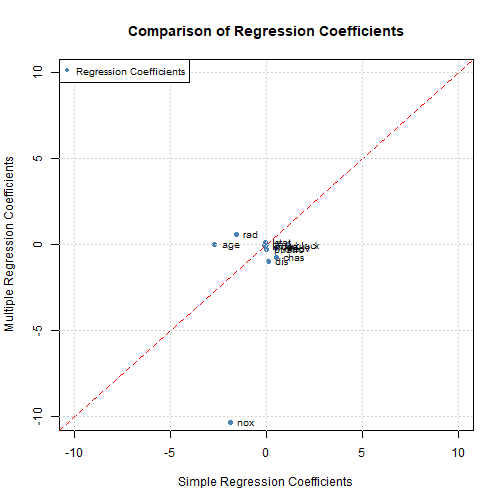
\includegraphics{hw1_files/figure-latex/problem3Code-1.pdf}

\hypertarget{question-4}{%
\subsection{Question 4}\label{question-4}}

\begin{Shaded}
\begin{Highlighting}[]
\CommentTok{\# Select variables of interest}
\NormalTok{variables\_of\_interest }\OtherTok{\textless{}{-}} \FunctionTok{c}\NormalTok{(}\StringTok{"zn"}\NormalTok{, }\StringTok{"dis"}\NormalTok{, }\StringTok{"rad"}\NormalTok{, }\StringTok{"black"}\NormalTok{, }\StringTok{"medv"}\NormalTok{)}

\CommentTok{\# Create an empty vector to store the p{-}values for the cubic model}
\NormalTok{p\_values\_cubic }\OtherTok{\textless{}{-}} \FunctionTok{vector}\NormalTok{(}\StringTok{"numeric"}\NormalTok{, }\AttributeTok{length =} \FunctionTok{length}\NormalTok{(variables\_of\_interest))}

\CommentTok{\# Fit cubic models for each variable}
\ControlFlowTok{for}\NormalTok{ (i }\ControlFlowTok{in} \DecValTok{1}\SpecialCharTok{:}\FunctionTok{length}\NormalTok{(variables\_of\_interest)) \{}
\NormalTok{  predictor }\OtherTok{\textless{}{-}}\NormalTok{ Boston[, variables\_of\_interest[i]]}
  
  \CommentTok{\# Fit the cubic model}
\NormalTok{  cubic\_model }\OtherTok{\textless{}{-}} \FunctionTok{lm}\NormalTok{(crim }\SpecialCharTok{\textasciitilde{}}\NormalTok{ predictor }\SpecialCharTok{+} \FunctionTok{I}\NormalTok{(predictor}\SpecialCharTok{\^{}}\DecValTok{2}\NormalTok{) }\SpecialCharTok{+} \FunctionTok{I}\NormalTok{(predictor}\SpecialCharTok{\^{}}\DecValTok{3}\NormalTok{), }\AttributeTok{data =}\NormalTok{ Boston)}
  
  \CommentTok{\# Extract the p{-}value for the cubic term}
\NormalTok{  p\_value }\OtherTok{\textless{}{-}} \FunctionTok{summary}\NormalTok{(cubic\_model)}\SpecialCharTok{$}\NormalTok{coefficients[}\DecValTok{4}\NormalTok{, }\StringTok{"Pr(\textgreater{}|t|)"}\NormalTok{]}
  
  \CommentTok{\# Store the p{-}value}
\NormalTok{  p\_values\_cubic[i] }\OtherTok{\textless{}{-}}\NormalTok{ p\_value}
  
  \CommentTok{\# Print the p{-}value for the cubic term}
  \FunctionTok{cat}\NormalTok{(}\StringTok{"Variable:"}\NormalTok{, variables\_of\_interest[i], }\StringTok{"}\SpecialCharTok{\textbackslash{}t}\StringTok{ p{-}value for cubic term:"}\NormalTok{, p\_value, }\StringTok{"}\SpecialCharTok{\textbackslash{}n}\StringTok{"}\NormalTok{)}
\NormalTok{\}}
\end{Highlighting}
\end{Shaded}

\begin{verbatim}
## Variable: zn      p-value for cubic term: 0.2295386 
## Variable: dis     p-value for cubic term: 1.088832e-08 
## Variable: rad     p-value for cubic term: 0.4823138 
## Variable: black   p-value for cubic term: 0.5436172 
## Variable: medv    p-value for cubic term: 1.04651e-12
\end{verbatim}

\begin{Shaded}
\begin{Highlighting}[]
\CommentTok{\# Identify variables with a significant cubic relationship}
\NormalTok{significant\_cubic\_predictors }\OtherTok{\textless{}{-}}\NormalTok{ variables\_of\_interest[p\_values\_cubic }\SpecialCharTok{\textless{}} \FloatTok{0.05}\NormalTok{]}

\CommentTok{\# Print the variables with a significant cubic relationship}
\FunctionTok{cat}\NormalTok{(}\StringTok{"}\SpecialCharTok{\textbackslash{}n}\StringTok{Variables with a significant cubic relationship:}\SpecialCharTok{\textbackslash{}n}\StringTok{"}\NormalTok{)}
\end{Highlighting}
\end{Shaded}

\begin{verbatim}
## 
## Variables with a significant cubic relationship:
\end{verbatim}

\begin{Shaded}
\begin{Highlighting}[]
\FunctionTok{cat}\NormalTok{(significant\_cubic\_predictors, }\AttributeTok{sep =} \StringTok{", "}\NormalTok{)}
\end{Highlighting}
\end{Shaded}

\begin{verbatim}
## dis, medv
\end{verbatim}

{[}In this code, we iterate over each predictor in the Boston dataset
and fit a cubic model using the lm() function. The model includes the
predictor, its squared term (I(predictor\^{}2)), and its cubed term
(I(predictor\^{}3)).

We then extract the p-value for the cubic term from the summary of the
cubic model using summary(cubic\_model)\$coefficients{[}4,
``Pr(\textgreater\textbar t\textbar)''{]} and store it in the
p\_values\_cubic vector.

The code prints the predictor name and its corresponding p-value for the
cubic term. A significant p-value (typically less than 0.05) indicates
evidence of a non-linear relationship between the predictor and the
response variable.

Finally, we identify the predictors with a significant cubic
relationship by filtering the names of the Boston dataset using
p\_values\_cubic \textless{} 0.05 and print them out.{]}

\end{document}
